% \usetikzlibrary{mindmap,backgrounds}
% \usetikzlibrary{decorations.pathmorphing}
% \usetikzlibrary{decorations.markings}
% \usetikzlibrary{arrows.meta,bending}

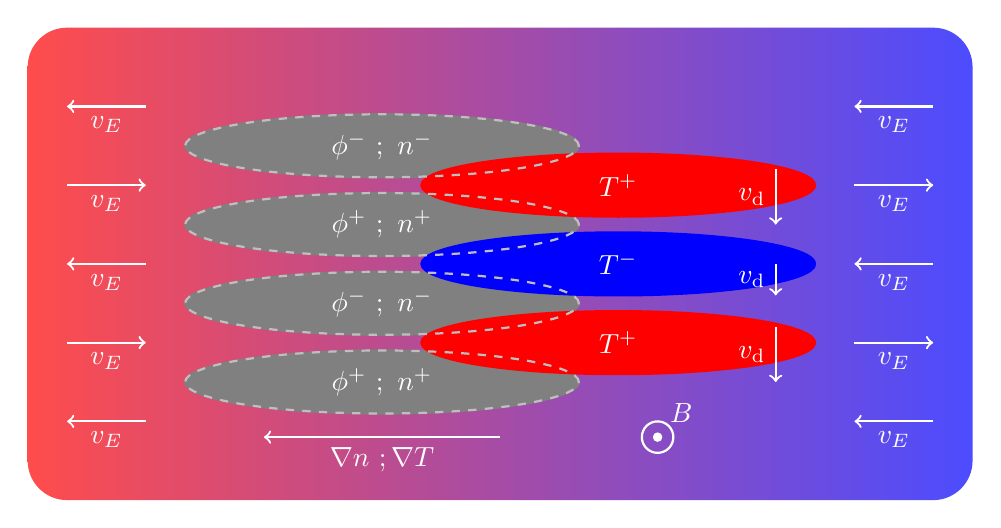
\begin{tikzpicture}
    % Temperature background
    \shade [left color=red, right color= blue, rounded corners = 0.5cm, opacity = 0.7] (0,0) rectangle (12,6);
    % Magnetic field
    \draw [thick, white] (8,0.8) circle (0.2);
    \filldraw [white] (8,0.8) circle (1.5pt);
    \draw (8.3,1.1) node[white]{$\vect{B}$};
    % Density and Potencial cells
    \draw [thick, gray, opacity=1, fill = gray] (4.5,4.5) ellipse (2.5 and 0.4) node[white, opacity=1]{$\phi^{-}~;~n^{-}$};
    \draw [thick, gray, opacity=1, fill = gray] (4.5,3.5) ellipse (2.5 and 0.4) node[white, opacity=1]{$\phi^{+}~;~n^{+}$};
    \draw [thick, gray, opacity=1, fill = gray] (4.5,2.5) ellipse (2.5 and 0.4) node[white, opacity=1]{$\phi^{-}~;~n^{-}$};
    \draw [thick, gray, opacity=1, fill = gray] (4.5,1.5) ellipse (2.5 and 0.4) node[white, opacity=1]{$\phi^{+}~;~n^{+}$};
    % Temperature cells
    \draw [thick, red, opacity=1, fill = red]   (7.5,4) ellipse (2.5 and 0.4) node[white, opacity=1]{$T^{+}$};
    \draw [thick, blue, opacity=1, fill = blue] (7.5,3) ellipse (2.5 and 0.4) node[white, opacity=1]{$T^{-}$};
    \draw [thick, red, opacity=1, fill = red]   (7.5,2) ellipse (2.5 and 0.4) node[white, opacity=1]{$T^{+}$};
    % Temperature and density gradient
    \draw[thick, white, <-] (3,0.8) -- (6,0.8) node[midway, below, white]{$\nabla n~;\nabla T$};
    % Outline Density and Potencial cell
    \draw [thick, lightgray, dashed] (4.5,4.5) ellipse (2.5 and 0.4);
    \draw [thick, lightgray, dashed] (4.5,3.5) ellipse (2.5 and 0.4);
    \draw [thick, lightgray, dashed] (4.5,2.5) ellipse (2.5 and 0.4);
    \draw [thick, lightgray, dashed] (4.5,1.5) ellipse (2.5 and 0.4);
    % Grad B and curvature drift velocity
    \draw[thick, white, ->] (9.5,4.2) -- (9.5,3.5) node[midway, left, white]{$\vect{v}_\mathrm{d}$};
    \draw[thick, white, ->] (9.5,3) -- (9.5,2.6) node[midway, left, white]{$\vect{v}_\mathrm{d}$};
    \draw[thick, white, ->] (9.5,2.2) -- (9.5,1.5) node[midway, left, white]{$\vect{v}_\mathrm{d}$};
    % ExB drift velocity
    \draw[thick, white, <-] (10.5,5) -- (11.5,5) node[midway, below, white]{$\vect{v}_{E}$};
    \draw[thick, white, ->] (10.5,4) -- (11.5,4) node[midway, below, white]{$\vect{v}_{E}$};
    \draw[thick, white, <-] (10.5,3) -- (11.5,3) node[midway, below, white]{$\vect{v}_{E}$};
    \draw[thick, white, ->] (10.5,2) -- (11.5,2) node[midway, below, white]{$\vect{v}_{E}$};
    \draw[thick, white, <-] (10.5,1) -- (11.5,1) node[midway, below, white]{$\vect{v}_{E}$};
    \draw[thick, white, <-] (0.5,5) --   (1.5,5) node[midway, below, white]{$\vect{v}_{E}$};
    \draw[thick, white, ->] (0.5,4) --   (1.5,4) node[midway, below, white]{$\vect{v}_{E}$};
    \draw[thick, white, <-] (0.5,3) --   (1.5,3) node[midway, below, white]{$\vect{v}_{E}$};
    \draw[thick, white, ->] (0.5,2) --   (1.5,2) node[midway, below, white]{$\vect{v}_{E}$};
    \draw[thick, white, <-] (0.5,1) --   (1.5,1) node[midway, below, white]{$\vect{v}_{E}$};
\end{tikzpicture}